\documentclass[12pt]{article}
\usepackage{setspace}
\usepackage{a4}
\usepackage{amssymb,amsmath,amsthm,latexsym}
\usepackage{amsfonts}
\usepackage{array}
\usepackage[numbers]{natbib}
\bibliographystyle{plainnat}
\usepackage{float}
\usepackage[nottoc]{tocbibind}
\setlength{\parindent}{1.0cm} \setlength{\evensidemargin}{0.0cm}
\setlength{\oddsidemargin}{0.0cm} \setlength{\topmargin}{0.0cm}

\textwidth 17cm \textheight 20cm
\onehalfspacing

\usepackage{microtype}
\usepackage{tablefootnote}
\usepackage{threeparttable}  
\usepackage{booktabs}
\usepackage{caption}
\captionsetup{justification   = raggedright,
              singlelinecheck = false}
\usepackage{bm}
\usepackage{stfloats}
\usepackage{mathrsfs}
\usepackage{tabularx}
\usepackage{multirow}
\usepackage{nicematrix}
\usepackage[thinlines]{easytable}
\usepackage{enumitem}
\usepackage{textcomp}
\usepackage{subcaption}

\usepackage{adjustbox}
\usepackage{graphicx}
\usepackage{tikz}
\usetikzlibrary{shapes.geometric, arrows, positioning}
\makeatletter
\usepackage{listings}
\usepackage{color}

\definecolor{dkgreen}{rgb}{0,0.6,0}
\definecolor{gray}{rgb}{0.5,0.5,0.5}
\definecolor{mauve}{rgb}{0.58,0,0.82}
\lstset{frame=tb,
  language=Python,
  aboveskip=3mm,
  belowskip=3mm,
  showstringspaces=false,
  columns=flexible,
  basicstyle={\small\ttfamily},
  numbers=none,
  numberstyle=\tiny\color{gray},
  keywordstyle=\color{blue},
  commentstyle=\color{dkgreen},
  stringstyle=\color{mauve},
  breaklines=true,
  breakatwhitespace=true,
}

\usepackage[justification=centering]{caption}

\usepackage{multicol}
\usepackage{longtable}

\usepackage{algorithm,algorithmic}
\def\newblock{\hskip .11em plus .33em minus .07em}
\def\BibTeX{{\rm B\kern-.05em{\sc i\kern-.025em b}\kern-.08em
		T\kern-.1667em\lower.7ex\hbox{E}\kern-.125emX}}

\AtBeginEnvironment{procedure}{\let\c@algocf\c@procedure}
\makeatother

\newtheorem{definition}{Definition}
\usepackage{etoolbox}
\newcounter{procedure}
\makeatletter
\AtBeginEnvironment{procedure}{\let\c@algocf\c@procedure}
\makeatother
\captionsetup[table]{labelsep=newline}
\captionsetup[figure]{labelsep=period}
\captionsetup[subfigure]{font=footnotesize}
\makeatletter
\xpatchcmd{\@thm}{\fontseries\mddefault\upshape}{}{}{} % same font as thm-header
\makeatother
\newtheorem{lemma}{Lemma}

\newcommand*{\comb}[2]{{}^{#1}C_{#2}}%
\newcommand{\RNum}[1]{\lowercase\expandafter{\romannumeral #1\relax}}
\makeatletter
\@dblfptop 0pt
\makeatother

\begin{document}
\begin{titlepage}
\doublespacing

\begin{center}
\par {\large \textbf{Mini Project Report}}\\
\end{center}

\begin{center}
	\par {\large \textbf{on}}
\end{center}

\begin{center}
{\Large \textbf{Intelligent Timetable Query System using Text-to-SQL RAG}}
\end{center}

{\small
\begin{center}
\par \small {Submitted by}
\par \Large \textbf{Student Names} \textbf{Reg. Numbers}
\par Under the guidance of
\par \large \textbf{Guide Name}
\par \textbf{Designation}
\end{center}
}

\begin{figure}[h]
\begin{center}
% \includegraphics[height=.80in]{iiIT-Dharwad-Logo-horizontal-500x154[1].png}
\end{center}
\end{figure}

\begin{center}
\par{\mbox {\small\textbf{DEPARTMENT OF COMPUTER SCIENCE AND ENGINEERING}}}
\noindent{\mbox{\small \textbf{ INDIAN INSTITUTE OF INFORMATION TECHNOLOGY
DHARWAD}}}\\
XX/XX/2024

\end{center}
\end{titlepage}

\newpage
\thispagestyle{empty}
\clearpage             
\thispagestyle{empty}  
\phantom{a}            
\newpage
\thispagestyle{empty}

\begin{center}	
	\emph{\huge{Certificate}}\\[2.5cm]
\end{center}
\normalsize This is to certify that the project, entitled \textbf{Intelligent Timetable Query System using Text-to-SQL RAG}, is a bonafide record of the Mini Project coursework presented by the students whose names are given below during 2024 in partial fulfilment of the requirements of the degree of Bachelor of Technology in Computer Science and Engineering.\\[1.0cm]

\begin{table}[h]
	\centering
	\begin{tabular}{lr}
		Roll No & Names of Students \\ \\ \hline
		\\
		Roll 1 & Name 1 \\ 
		Roll 2 & Name 2 \\ 
		Roll 3 & Name 3 \\ 
	\end{tabular}
\end{table}

\vfill

\begin{flushright}
	Guide Name\\
	(Project Supervisor )\\[1.5cm]
\end{flushright}

\newpage
\pagenumbering{roman}
\setcounter{page}{1}
\tableofcontents
\newpage


\newpage
\thispagestyle{empty}
\clearpage             
\thispagestyle{empty}  
\phantom{a}            
\newpage

\section{Introduction}
\pagenumbering{arabic}
\subsection{Motivation}
In modern academic institutions, course timetables often comprise complex matrices of subjects, faculties, room numbers, and timings across several different branches and semesters. As the scale of an institution grows, the dimensionality of this scheduling data becomes increasingly difficult to manage and navigate using standard analog or static digital formats. Students and faculty frequently find themselves scrolling through dense, hard-to-read CSV or PDF files simply to answer a trivial scheduling question like finding their next class. 

\subsection{Problem Statement}
Existing timetable distribution methods are static and cumbersome. Most institutions rely on distributing Excel spreadsheets or PDFs every semester. Consequently, finding a specific class time, locating a particular faculty member, or checking the schedule for a specific day becomes a tedious search task. While some rule-based chatbots have been deployed for these tasks, they suffer from rigid dialogue trees and often fail when users deviate from expected syntax.

\subsection{Objectives}
To address these challenges, this project introduces an \textbf{Intelligent Timetable Query System} built on a Text-to-SQL Retrieval-Augmented Generation (RAG) architecture. The objective of this system is to bridge the gap between natural language processing and structured database querying. By allowing students to interactively ask plain English questions—such as \textit{"When is my Data Structures class on Monday?"} or \textit{"Which faculty is teaching the morning first session?"}—the system aims to provide instance, factual, and correct responses by evaluating those questions directly against a backend SQL database containing the timetable data.

\newpage

\section{Literature Review}

\subsection{Evolution of Academic Scheduling Systems}
Traditional approaches to academic scheduling and timetable sharing heavily revolve around digital distribution in the form of Excel spreadsheets or PDF documents. The static nature of these documents introduces friction whenever rapid lookup is required. As early academic portals evolved, web interfaces began providing filtered tabular views, but this still required users to manually select branches, semesters, and days from multiple dropdown menus.

\subsection{Limitations of Rule-based Chatbots}
With the rise of conversational AI, universities began deploying rule-based chatbots. These systems mapping specific keywords to predefined static responses. However, rule-based systems are extremely fragile; they lack the flexibility to handle complex, chained, or lexically nuanced questions and require developers to manually maintain extensive dialogue trees for every edge case.

\subsection{Retrieval-Augmented Generation (RAG)}
Recently, the advent of Large Language Models (LLMs) like GPT-4 and Gemini has given rise to the Retrieval-Augmented Generation (RAG) paradigm \cite{rag_paper}. Standard RAG operates by retrieving unstructured text chunks based on the cosine similarity of vector embeddings, and then synthesizing an answer via an LLM. While highly effective for document analysis, standard RAG struggles with structured tabular data, frequently hallucinating row/column relationships or failing basic aggregation tasks.

\subsection{Text-to-SQL Paradigms}
To counteract the weaknesses of standard RAG over structured data, researchers have introduced Text-to-SQL pipelines \cite{llm_sql}. Instead of providing the LLM with the data itself, the LLM is provided only with the \textit{schema} of the database. The model generates an exact SQL query based on the user's natural language input. By directly executing exact database queries on a backend engine, the system entirely removes the risk of LLM hallucinations regarding factual data. Our work adapts this state-of-the-art methodology explicitly to the problem of university timetable management.

\newpage

\section{System Architecture and Methodology}  

\subsection{High-Level Design}
Our platform is designed as a three-tier modern decoupled microservices architecture composed of a Next.js front-end application, a Spring Boot API Gateway and Authentication layer, and a Python FastAPI backend service. The entire query-response workflow is structured into logical stages across these microservices:
\begin{enumerate}
    \item \textbf{Frontend Interaction (Next.js):} The client-side application captures user authentication and submits natural language timetable questions.
    \item \textbf{Authentication \& Routing (Spring Boot):} Incoming requests are intercepted by a Spring Security JWT Filter. The Java middleware authenticates the token, checks constraints securely, and proxies valid AI queries to the FastAPI service.
    \item \textbf{Schema Extraction (FastAPI):} The Python AI backend receives the proxy-forwarded request, identifies the pertinent database table utilizing contextual parameters, and retrieves its exact SQL schema.
    \item \textbf{Text-to-SQL Generation:} A Google Gemini LLM processes the user's question and schema context to generate a robust SQLite query over the network.
    \item \textbf{Database Execution:} The generated SQL runs locally against the timetable database.
    \item \textbf{Explanation Synthesis:} The LLM receives the SQL results and formulates a conversational English response, which is routed back through the Spring Boot proxy to the Next.js client.
\end{enumerate}

\begin{figure}[H]
\centering
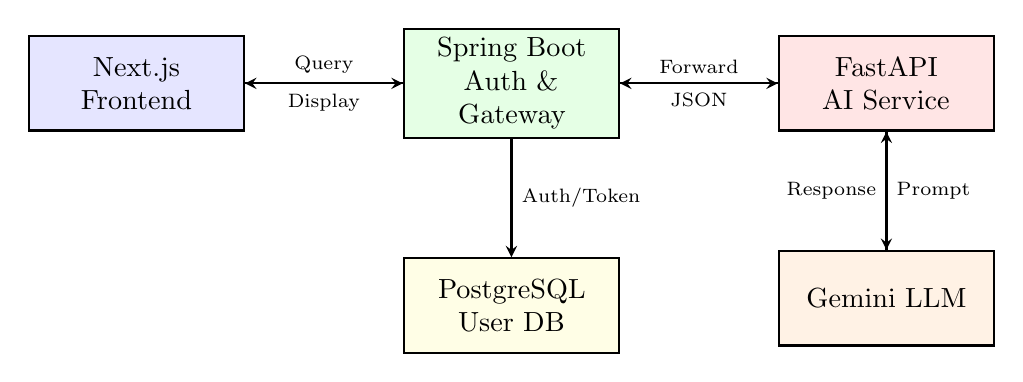
\begin{tikzpicture}[
  node distance=1.5cm and 2cm,
  box/.style={rectangle, draw=black, thick, fill=blue!10, text width=2.5cm, align=center, minimum height=1.2cm},
  arrow/.style={thick,->,>=stealth}
]
\node (client) [box] {Next.js \\ Frontend};
\node (auth) [box, right=of client, fill=green!10] {Spring Boot \\ Auth \& Gateway};
\node (ai) [box, right=of auth, fill=red!10] {FastAPI \\ AI Service};
\node (db) [box, below=of auth, fill=yellow!10] {PostgreSQL \\ User DB};
\node (llm) [box, below=of ai, fill=orange!10] {Gemini LLM};

\draw [arrow] (client) -- node[above]{\scriptsize Query} (auth);
\draw [arrow] (auth) -- node[above]{\scriptsize Forward} (ai);
\draw [arrow] (auth) -- node[right]{\scriptsize Auth/Token} (db);
\draw [arrow] (ai) -- node[right]{\scriptsize Prompt} (llm);
\draw [arrow, dashed] (llm) -- node[left]{\scriptsize Response} (ai);
\draw [arrow, dashed] (ai) -- node[below]{\scriptsize JSON} (auth);
\draw [arrow, dashed] (auth) -- node[below]{\scriptsize Display} (client);
\end{tikzpicture}
\caption{System Architecture Flow diagram representing microservices communication and Text-to-SQL mapping.}
\end{figure}

\subsection{Data Management and Database Schema}
Scheduling scheduling data is initially aggregated via institutional spreadsheets and subsequently transformed into normalized CSV files. A Python-based Extract, Transform, Load (ETL) script parses these CSVs to populate \textit{timetable.db}, a structured SQLite database. 

The tables are granularly separated by semester and branch (e.g., \textit{timetable\_sem4\_cse}, \textit{timetable\_sem6\_ds}). Each table holds attributes defining the \texttt{Day}, timeslots (e.g., \texttt{09:00-10:00}), subject codes, subject names, and the assigned professor. This normalization ensures rapid row-level lookup constraints.

\newpage

\section{Implementation Details}

\subsection{Technology Stack}
\begin{itemize}
    \item \textbf{Frontend Application:} Developed using Next.js (React) and styled with Tailwind CSS. The user interface features secure authentication screens and an intuitive chat interface.
    \item \textbf{Middleware \& Authentication:} Engineered in Java utilizing the Spring Boot framework. This layer leverages Spring Security and \textit{jjwt} for robust JWT-based authorization and interacts with a PostgreSQL database to persist user credentials. 
    \item \textbf{Backend Service:} Engineered in Python 3.10 and powered by the FastAPI framework to ensure asynchronous, low-latency API communication with the generative models.
    \item \textbf{Database Layers:} PostgreSQL is used for high-availability user management, while SQLite 3 provides serverless querying for the timetable AI semantic extraction.
    \item \textbf{AI Modeling:} Google GenAI APIs provide access to Gemini LLMs for reasoning and Text-to-SQL code generation.
\end{itemize}

\subsection{Prompt Engineering and Query Normalization}
A core component of the system relies on strict prompt engineering to maintain high fidelity in SQL generation. The generative prompt is injected with the extracted schema, formatted dynamically (e.g., \texttt{ColumnName (Datatype)}). 

To ensure resilience against colloquial inputs, rigid normalization rules are passed to the model:
\begin{lstlisting}[language=Python]
IMPORTANT NORMALIZATION RULES:
1. Convert abbreviated weekdays to full names (e.g., Mon -> Monday).
2. For dates (e.g., Feb 28), calculate resolving weekday.
3. For relative days ("today", "tomorrow"), compute corresponding days.
4. The database column "Day" ALWAYS stores full weekday names.
\end{lstlisting}
By enforcing that the model "thinks" through the normalization steps before writing the SQL clause, we drastically decrease syntax errors related to \texttt{WHERE} clauses matching abbreviations against full table string records.

\newpage

\section{Results and Discussions}  

\subsection{Efficacy and Hallucination Avoidance}
The developed full-stack application successfully interprets diverse user queries regardless of varying sentence structures. Because the pipeline splits query generation from final data execution, the responses are deterministic against the backend timetable database. Therefore, the architectural design mathematically guarantees absolute factual correctness while remaining dialogue-friendly, solving the hallucination problem inherent to classical RAG systems applied to tabular structures.

\subsection{Latency and Performance Metrics}
\textbf{Latency Observations:} Each incoming user request executes a two-hop path over the network connecting to the LLM API twice (once for SQL generation, once for synthesis). Therefore, the overall system response time is bounded significantly by external network bandwidth rather than local database I/O. However, even with sequential API calls, response synthesis typically triggers within $2$ to $4$ seconds. For student end-users, waiting $3$ seconds is still a magnitude faster than manually isolating rows on a PDF document.

\subsection{Sample Interaction Capabilities}
The model's ability to chain logical constraints was evaluated extensively. Below is a subset table illustrating the system's mapping capacity from natural query to executed SQL.

\begin{table}[H]
\centering
\begin{tabular}{|p{5cm}|p{6.5cm}|p{3.5cm}|}
\hline
\textbf{User Query} & \textbf{Generated SQL Concept} & \textbf{Outcome/Result} \\ \hline
"What classes do I have on Mon?" & \texttt{SELECT * FROM [...] WHERE Day='Monday'} & Succesful extraction of Monday schedule. \\ \hline
"Who teaches DBMS?" & \texttt{SELECT Faculty FROM [...] WHERE Subject LIKE '\%DBMS\%'} & Returns specific assigned professor. \\ \hline
"When is the break?" & \texttt{SELECT Time FROM [...] WHERE Subject='Break'} & Pinpoints chronological break parameters. \\ \hline
\end{tabular}
\caption{Sample cases showcasing query mapping robustness.}
\end{table}

\subsection{Edge Case Management}
A notable edge case involved vaguely phrased prompts that referenced colloquial class names rather than strict database mappings. The combination of the SQL \texttt{LIKE} statements enforced by the LLM prompt and the normalization parsing engine ensures the system safely navigates around ambiguous phrasing.

\newpage
  
\section{Conclusion and Future Scope}  

\subsection{Conclusion}
This project successfully designed, built, and implemented a novel timetable querying platform, effectively demonstrating the immense potential of Text-to-SQL workflows in linking human-centric questioning with structured institutional databases. By coordinating a Next.js user interface parallel to an asynchronous Python FastAPI backend, our application ensures a decoupled architecture scalable to university-wide loads. Google's Gemini models reliably translate complex English intents into executable relational algebra (SQL) and consequently construct concise, conversational answers for the user.

\subsection{Future Enhancements}
While highly functional, the architecture has avenues for continuous improvement:
\begin{itemize}
    \item \textbf{Local LLM Integration:} Transitioning the SQL generation step from a cloud API to a locally quantized, finetuned model (e.g., Llama-3-SQL) to eliminate network latency and drop query times into the sub-second range.
    \item \textbf{Aggressive Caching Layer:} Adopting a Redis caching layer to save previous NLP vectors against generated SQL pairs, effectively intercepting redundant API calls for commonly asked questions ("What is the first class tomorrow?").
    \item \textbf{Multi-turn Memory:} Expanding the synthesis agent with chat history arrays, enabling follow-up conversational flows regarding the student's timetable schedules without restating context.
\end{itemize}

\newpage
  
%%%***************************************************************************************  
\settocbibname{References}

\begin{thebibliography}{9}

\bibitem{llm_sql}
Rajkumar, P., Lee, R., \& Polozov, O. (2022). 
Evaluating Large Language Models on Text-to-SQL tasks. 
\textit{arXiv preprint arXiv:2204.00498}.

\bibitem{rag_paper}
Lewis, P., Perez, E., Piktus, A., Petroni, F., Karpukhin, V., Goyal, N., ... \& Yih, W. T. (2020). 
Retrieval-augmented generation for knowledge-intensive NLP tasks. 
\textit{Advances in Neural Information Processing Systems}, 33, 9459-9474.

\bibitem{fastapi}
FastAPI Framework Documentation. (2024). 
Available at \textit{https://fastapi.tiangolo.com/}.

\bibitem{nextjs}
Next.js Framework Documentation. (2024). 
Available at \textit{https://nextjs.org/docs}.

\end{thebibliography}

\end{document}
